\documentclass[10pt,twocolumn,letterpaper]{article}

\usepackage{cvpr}
\usepackage{times}
\usepackage{epsfig}
\usepackage{graphicx}
\usepackage{amsmath}
\usepackage{amssymb}
\usepackage{booktabs}

\usepackage[breaklinks=true,bookmarks=false]{hyperref}

\cvprfinalcopy % *** Uncomment this line for the final submission

\def\cvprPaperID{****}
\def\httilde{\mbox{\tt\raisebox{-.5ex}{\symbol{126}}}}

\setcounter{page}{1}
\begin{document}

%%%%%%%%% TITLE
\title{Scaling Drifting VQ-VAE to Real Images:\\
A Physics-Inspired Quantizer that Uses the Whole Codebook}

\author{Hemal Arora\\
Stanford University\\
{\tt\small hemal1@stanford.edu}
\and
Tesvara Jiang\\
Stanford University\\
{\tt\small tesvaraj@stanford.edu}
\and
Ethan Zhang\\
Stanford University\\
{\tt\small ez26@stanford.edu}
}

\maketitle

%%%%%%%%% ABSTRACT
\begin{abstract}
State-of-the-art image generators from VQGAN to DALL-E represent each image as a sequence of discrete codebook tokens, then generate new images by sampling new token sequences. As a result, codebook quality sets a hard ceiling on everything downstream, but in most codebooks, a few tokens carry the information while the rest sit idle. We study \emph{DriftingVQ}, which discards the standard codebook losses and instead treats encoder outputs and codewords as charged particles, so attraction pulls codes toward the data and repulsion spreads them apart. The method was proposed by researcher Ziming Liu only for a two-dimensional synthetic setting~\cite{liu2026drift}; whether it transfers to deep convolutional networks and real images was unknown. We found that the original DriftingVQ formulation underperforms a modern exponential-moving-average (EMA) baseline by $1.5$ to $2$\,dB. However, a component-wise ablation identified two fixes. By dropping a hidden-to-hidden repulsion term and adopting a straight-through gradient estimator, we reversed the gap. The resulting Drift$\star$ beats EMA on CIFAR-10 by $0.77$\,dB PSNR, $11.6$ FID points, and $3{\times}$ codebook perplexity, with consistent gains across CIFAR-100, STL-10, and Tiny ImageNet. Effective code usage holds near $80\%$ as the codebook grows to $8192$ entries, versus $22$ to $37\%$ for EMA. Downstream, Drift$\star$ codes improve both recognition and generation, though their higher entropy makes them harder for a prior to model. We show that codebook uniformity and reconstruction quality are not in conflict, suggesting future image generators can use larger, more expressive codebooks without losing fidelity.
\end{abstract}

%%%%%%%%% BODY TEXT
\section{Introduction}

Modern image and video generators work by first compressing each image into a small grid of discrete tokens from a learned codebook, and then generate new images by sampling new token sequences. The system pairs a vector-quantized autoencoder (VQ-VAE) with an autoregressive or diffusion prior in models like VQGAN and DALL$\cdot$E \cite{vqvae,vqgan,dalle}. Since the codebook is the vocabulary for everything downstream, its quality sets a hard ceiling on all downstream tasks.

In a standard VQ-VAE only the codeword nearest each encoder output receives a learning signal, so codes that start far from the data are never selected nor updated, which is called \emph{codebook collapse}. Sometimes thousands of codes act like a few hundred. Exponential-moving-average (EMA) trick revives dead codes but are still suboptimal because live codes are used in a Zipfian way, where only a few of them dominate. A $512$-entry EMA codebook can report $99.8\%$ of its codes ``active'' but, in entropy terms, maybe only about $136$ of them are actually helpful.

Liu \cite{liu2026drift} recently proposed a physics-inspired fix: drop the codebook and commitment losses and treat encoder outputs and codewords as charged particles, adding a pairwise \emph{potential energy} to the objective. Opposite charges attract, pulling codes onto the data and reviving unused ones. Like charges repel, spreading them evenly. The idea was shown only on a two-dimensional toy dataset with a linear encoder and decoder, so we wondered whether it survives deep convolutional networks and real images.

The original DriftingVQ does not. A faithful implementation reconstructs $1.5$ to $2$\,dB worse than EMA. But we did a component-wise ablation and isolated two components that consistently hurt. Removing them closed the gap, improving reconstruction (PSNR), perceptual quality (FID), and codebook usage. The gain is largest for big codebooks where standard quantizers waste the most capacity. In this paper, we explain the mechanism, evaluate the codes downstream, and mark where the method breaks. Our takeaway is that greater codebook utilization means more visual patters are learned. We show that advantage carries through to reconstruction, generation, and feature discriminability.

\section{Related Work}

\noindent\textbf{Vector-quantized autoencoders.} VQ-VAE \cite{vqvae} introduced
discrete latent codes, trained with a straight-through estimator (STE) alongside a
codebook and commitment loss. VQGAN \cite{vqgan} scaled the idea to high-resolution
synthesis with adversarial and perceptual losses, and discrete tokens now feed
text-to-image models \cite{dalle}. The codebook is updated either by gradient (the
``classical'' route) or, more commonly today, by an EMA of the assigned encoder
outputs.

\noindent\textbf{Fighting codebook collapse.} Codebook underuse is a recurring
problem. Common remedies revive dead codes by re-seeding them from recent encoder
outputs, or reparameterize the codebook, as in SimVQ \cite{simvq},
which routes all codes through one shared linear layer so that updating any code
nudges the rest. These methods raise \emph{utilization}, the fraction of codes used at
least once, but as we show that is a weak proxy: it misses the Zipfian concentration
that limits EMA. DriftingVQ \cite{liu2026drift} instead makes even usage an explicit
force in the loss. To our knowledge, this is the first evaluation of the approach
beyond its original two-dimensional toy example.

\noindent\textbf{Gradient estimators.} Nearest-neighbor assignment is not
differentiable, so VQ methods need a surrogate gradient for the encoder. The classic
choice is the STE \cite{vqvae}, which copies the gradient from the quantized output
straight to the encoder input. The rotation trick \cite{rotationtrick} instead rotates
the encoder output onto its assigned codeword for a lower-variance estimate. We find
that for this energy-based quantizer the simpler STE works better.

\section{Data}

We evaluate on a ladder of datasets that grows in difficulty, so that we can study
how the method scales rather than reporting a single operating point. All images
are mapped to a square latent grid (Section~\ref{sec:methods}) and pixel values are
scaled to $[-1,1]$. We apply random horizontal flips and no other augmentation.

\begin{itemize}\itemsep2pt
  \item \textbf{CIFAR-10 and CIFAR-100} \cite{cifar} have $50$k train and $10$k
  test natural images at $32{\times}32$. CIFAR-100 has $100$ classes versus
  CIFAR-10's $10$, and the wider class distribution makes the codebook's job harder.
  CIFAR-100 is our main testbed for scaling the codebook size $K$.
  \item \textbf{STL-10} \cite{stl10} has $100$k unlabeled images, originally
  $96{\times}96$, which we resize to $64{\times}64$. It has higher resolution and
  more visual variety than CIFAR, which makes it useful for the downstream study in
  Section~\ref{sec:downstream}.
  \item \textbf{Tiny ImageNet} \cite{tinyimagenet} has $200$ classes at
  $64{\times}64$ with $100$k train images, and is the hardest reconstruction target
  we use.
\end{itemize}

\noindent Reconstruction quality is measured on the held-out test split, and FID is
computed between test images and their reconstructions.

\section{Methods}
\label{sec:methods}

\subsection{Shared autoencoder, swappable quantizer}

To keep the comparison fair, we fix one convolutional autoencoder and swap only the
quantizer in the middle. The encoder is a small residual CNN: a convolutional stem,
strided downsampling blocks, and residual blocks with GroupNorm and SiLU activations.
It maps each image to an $8{\times}8$ grid of $d{=}64$-dimensional latent vectors, and
the decoder mirrors it. CIFAR images use two downsampling stages ($32{\to}8$); the
$64{\times}64$ datasets use three. The quantizer takes the $8{\times}8{\times}64$
feature map, replaces each spatial vector with its nearest codebook entry, and returns
the quantized map, the index assignment, and any quantizer-specific
loss.\footnote{Our quantizer implementations build on the open-source
\texttt{vector-quantize-pytorch} library (github.com/lucidrains/vector-quantize-pytorch).}

Since the encoder, decoder, and training budget are identical everywhere, any
difference in results comes from the quantizer alone. We train with AdamW (learning
rate $3\!\times\!10^{-4}$, batch size $128$). The training objective is
\begin{equation}
\mathcal{L} = \|x - \hat{x}\|^2 + \mathcal{L}_{\mathrm{quant}},
\label{eq:objective}
\end{equation}
a reconstruction term plus a quantizer-specific loss $\mathcal{L}_{\mathrm{quant}}$,
where $x$ is the input image and $\hat{x}$ its reconstruction.

\subsection{Baselines}
\label{sec:baselines}

We compare against three standard quantizers.

\noindent\textbf{EMA.} Each codeword is an exponential moving average of the encoder
outputs assigned to it:
\begin{equation}
e_k \;\leftarrow\; m\,e_k + (1-m)\,\bar{z}_k,
\label{eq:ema}
\end{equation}
where $\bar{z}_k$ is the mean encoder output assigned to code $k$ in the batch and $m$
is the decay rate. No gradient reaches the codebook; the encoder learns through the
reconstruction loss alone. This is the default in modern VQ-VAEs and our primary
baseline.

\noindent\textbf{Classical.} The codebook is trained by gradient descent with a
codebook loss and a commitment loss,
\begin{equation}
\mathcal{L}_{\mathrm{classical}} = \|\mathrm{sg}[z_e] - e\|^2 + \beta\,\|z_e - \mathrm{sg}[e]\|^2,
\label{eq:classical}
\end{equation}
where $z_e$ is the encoder output, $e$ the nearest codeword, $\mathrm{sg}[\cdot]$ the
stop-gradient operator, and $\beta{=}0.25$. The first term pulls each codeword toward
its assigned outputs; the second pulls the outputs back toward the codeword (the
commitment penalty).

\noindent\textbf{SimVQ.} Every codeword is a shared linear projection of a fixed random
vector,
\begin{equation}
e_k = W c_k,
\label{eq:simvq}
\end{equation}
where the $\{c_k\}_{k=1}^K$ are fixed at initialization and $W$ is a single learned
matrix~\cite{simvq}. Because all codes share $W$, one gradient step shifts the whole
codebook at once, which keeps individual codes from drifting into unused regions.

\subsection{DriftingVQ}
\label{sec:driftingvq}

DriftingVQ \cite{liu2026drift} drops the codebook and commitment losses entirely.
It first projects every encoder output (a ``hidden'') and every codeword onto the unit
sphere with $L_2$ normalization, then treats them as point charges: each of the $N$
hiddens carries charge $+1/N$ and each of the $K$ codes carries $-1/K$, so the system
is neutral overall. Every pair of charges interacts through the potential
\begin{equation}
U(r) = \tau\,(r+\tau)\,e^{-r/\tau}\,q_1 q_2,
\label{eq:potential}
\end{equation}
where $r$ is the distance between two points and $\tau$ is an interaction length scale.
On the unit sphere $r$ lies in $[0,2]$, so a given $\tau$ means the same thing across
runs. The sign of $q_1 q_2$ does the rest: opposite charges attract, like charges
repel. Summing over the three kinds of pairs gives the three terms of
$\mathcal{L}_{\mathrm{quant}}$:
\begin{itemize}\itemsep1pt
  \item $U_{pn}$: hidden-to-code attraction, which pulls codes toward the data and
  revives unused ones. Cost $O(NK)$.
  \item $U_{nn}$: code-to-code repulsion, which spreads codes apart and prevents
  collapse. Cost $O(K^2)$.
  \item $U_{pp}$: hidden-to-hidden repulsion, which pushes encoder outputs apart. Cost
  $O(N^2)$, estimated on a random subsample.
\end{itemize}
The original method sums all three and passes the encoder gradient through the
\emph{rotation trick}~\cite{rotationtrick}, which rotates the encoder output onto its
nearest codeword for a lower-variance estimate:
\begin{equation}
E_{\mathrm{orig}} = U_{pp} + U_{nn} + U_{pn}.
\label{eq:eliu}
\end{equation}
Our variant, Drift$\star$, drops the hidden-to-hidden term and uses a plain
\emph{straight-through estimator} (STE) instead, copying the gradient from the
quantized output back through the nearest-neighbor lookup to the encoder:
\begin{equation}
E_{\star} = U_{nn} + U_{pn}.
\label{eq:estar}
\end{equation}
Both choices come from the ablation in Section~\ref{sec:ablation}.

\subsection{From the original method to Drift$\star$}

Our main methodological contribution is figuring out which parts of this recipe to
keep. We changed one ingredient at a time (Section~\ref{sec:ablation}) and landed on
Drift$\star$: keep $U_{nn}$, $U_{pn}$, and $L_2$ normalization; drop $U_{pp}$; and
swap the rotation trick for STE, with $\tau{=}1.0$ and energy weight $1.0$. Briefly,
$U_{pp}$ makes the encoder spread its outputs apart for reasons unrelated to
reconstruction, which costs image quality, and the rotation trick, despite its lower
variance in theory, did worse here in practice.

\subsection{Metrics, and why utilization misleads}

We report four reconstruction metrics. \emph{PSNR} (in dB) measures pixel-level
fidelity, where a $1$\,dB gain is a visible improvement in fine detail. \emph{SSIM}
measures structural similarity. \emph{LPIPS}~\cite{lpips} measures perceptual
similarity through deep features, with lower meaning closer to a human eye.
\emph{FID}~\cite{fid} measures how far the reconstructed images are from the real ones
as distributions, again lower is better. In all tables $\uparrow$ means higher is
better, $\downarrow$ means lower is better, and bold marks the better result in each
row.

For codebook usage we report three statistics and lean on the last two.
\emph{Utilization} is the fraction of codes used at least once in a batch.
\emph{Perplexity} is $\exp(H)$, the exponential of the usage-distribution entropy $H$,
ranging from $1$ to $K$; loosely, the effective number of codes in use. The \emph{Gini
coefficient} runs from $0$ for perfectly even usage to $1$ for maximal concentration.
Utilization on its own misleads: EMA routinely tops $95\%$ while perplexity sits far
below $K$, because a few codes absorb most of the assignments. We therefore also report
\textbf{ppl/$K$}, perplexity divided by codebook size, where a value near $1$ means
near-uniform usage and a value near $0$ means heavy concentration on a few codes.

\section{Experiments}

\subsection{The main result}
\label{sec:main}

Our main comparison is CIFAR-10 at $K{=}512$, trained to convergence ($30$k iterations, mean $\pm$ std over $3$ seeds). Table~\ref{tab:headline} shows Drift$\star$ ahead of the EMA baseline on all three axes at once, with higher PSNR, lower FID, and more even codebook usage. The gap is modest but consistent, about $0.77$\,dB PSNR and $11.6$ FID, and the codebook is used roughly three times more evenly. Figure~\ref{fig:usage} makes the usage difference visible. While EMA concentrates assignments on a small fraction of its codes, Drift$\star$ is closer to uniform.


\begin{table}[ht]
\centering\small
\setlength{\tabcolsep}{4pt}
\resizebox{\columnwidth}{!}{%
\begin{tabular}{lccccc}
\toprule
Method & PSNR$\uparrow$ & FID$\downarrow$ & LPIPS$\downarrow$ & ppl$\uparrow$ & Gini$\downarrow$\\
\midrule
\textbf{Drift$\star$} (no $U_{pp}$, STE) & \textbf{24.15} & \textbf{48.2} & \textbf{0.203} & 409 & 0.37\\
\quad no $U_{pp}$, rot.\ trick & 24.10 & 49.8 & 0.204 & 410 & 0.36\\
\quad with $U_{pp}$, STE & 23.98 & 49.3 & 0.210 & 466 & 0.24\\
\quad with $U_{pp}$, rot.\ trick & 23.20 & 60.1 & 0.244 & 490 & 0.16\\
\midrule
EMA (baseline) & 23.39 & 59.8 & 0.247 & 136 & 0.74\\
Classical & 22.98 & 65.0 & 0.266 & 106 & 0.75\\
SimVQ & 21.94 & 76.4 & 0.306 & 59 & 0.86\\
\bottomrule
\end{tabular}%
}
\vspace{2mm}
\caption{Main comparison on CIFAR-10, $K{=}512$, $30$k iters, $3$ seeds. The four
DriftingVQ rows form a $2{\times}2$ ablation over the two key changes: removing
$U_{pp}$ and switching from the rotation trick to STE. The original formulation
(row 4) reaches high perplexity but does not beat EMA on reconstruction; each change
helps on its own, and combining both gives Drift$\star$.}
\label{tab:headline}
\end{table}

\begin{figure}[ht]
\centering
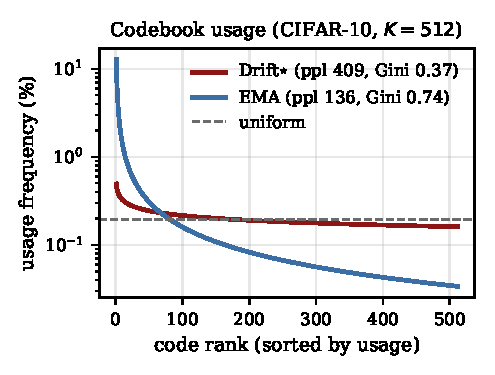
\includegraphics[width=0.92\linewidth]{figures/usage_dist.pdf}
\caption{Illustrative code-usage distributions for CIFAR-10, $K{=}512$, generated
to match the perplexity and Gini values measured from trained models
(Table~\ref{tab:headline}). Frequencies are sorted from most to least used (log
scale). EMA concentrates the majority of assignments on a small fraction of its
$512$ codes; Drift$\star$ is close to uniform.}
\label{fig:usage}
\end{figure}

\subsection{Qualitative reconstructions}
\label{sec:qualitative}

Figure~\ref{fig:recons} shows reconstructions on held-out test images, with input, EMA,
and Drift$\star$ side by side. With the encoder, decoder, and training budget fixed,
any visible difference is down to the quantizer. Drift$\star$ tends to hold onto finer
detail, edges, textures, and small structures, where EMA more often smooths them over.
Mean PSNR on these images is $24.3$\,dB for EMA and $25.2$\,dB for Drift$\star$, which
is consistent with a more evenly used codebook having more distinct codes to spend on
detail rather than routing many different patches through the same few popular ones.


\begin{figure}[ht]
\centering
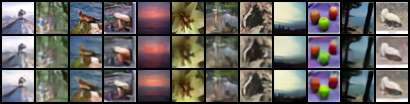
\includegraphics[width=\linewidth]{figures/recon_compare_cifar.png}
\caption{Reconstructions on held-out CIFAR-100 test images ($K{=}512$). Top row:
input. Middle row: EMA reconstruction. Bottom row: Drift$\star$ reconstruction,
all on the same images. Drift$\star$ preserves slightly more fine detail where EMA
tends to blur. The difference is subtle at $32{\times}32$, motivating the
higher-resolution study in Section~\ref{sec:stl10}.}
\label{fig:recons}
\end{figure}

\subsection{Ablation: which ingredients matter}
\label{sec:ablation}

The result in Table~\ref{tab:headline} comes out of an ablation that isolates each
ingredient. Starting from the full original method, we changed one component at a time
(CIFAR-10, $K{=}512$, $10$k iters, seed $0$; EMA scores $23.53$\,dB and $60.9$ FID at
this budget). Figure~\ref{fig:ablation} plots the PSNR change against EMA. Four things
stand out.

\begin{figure}[ht]
\centering
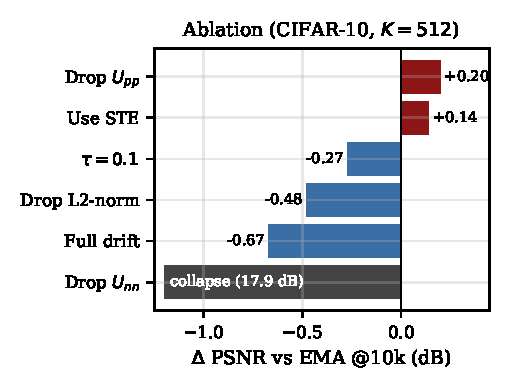
\includegraphics[width=0.95\linewidth]{figures/ablation.pdf}
\caption{Ablation of DriftingVQ ingredients, shown as PSNR change versus the EMA
baseline at $10$k iterations. Dropping $U_{pp}$ and switching to STE each move the
method above EMA; dropping $U_{nn}$ collapses the codebook entirely.}
\label{fig:ablation}
\end{figure}

\noindent\textbf{(1) $U_{pp}$ hurts, so we remove it.} Dropping the hidden-to-hidden
repulsion gains $0.87$\,dB over the full original method and lands $0.20$\,dB above
EMA. The term makes the encoder spread its outputs apart for reasons unrelated to
reconstruction, which appears to work against image quality.

\noindent\textbf{(2) STE does better than the rotation trick here.} Swapping the
rotation-trick gradient for a plain STE gains $0.81$\,dB and cuts FID by $10.7$ at
$10$k iterations. The rotation trick has lower variance in theory, but the STE was
consistently better in our runs.

\noindent\textbf{(3) $U_{nn}$ is load-bearing.} This is the one term we cannot drop.
Removing it collapses the codebook to $79$ of $512$ active codes and PSNR to
$17.9$\,dB. Without code-to-code repulsion, the codes pile onto the data and onto each
other.

\noindent\textbf{(4) $L_2$ normalization and $\tau$.} Removing $L_2$ normalization
costs $0.48$\,dB. The interaction scale $\tau$ has to be large enough for the energy to
turn on (Section~\ref{sec:mech}), and below about $\tau{=}0.3$ the forces effectively
vanish.

Combining the two helpful changes, dropping $U_{pp}$ and using STE, gives Drift$\star$.
A sweep over $\tau$ and energy weight (Table~\ref{tab:sweep}) confirms the defaults.
One thing we noticed is that the best $\tau$ for Drift$\star$ ($1.0$) sits at the
opposite end of the range from the best $\tau$ for the original method ($0.1$), which
suggests removing $U_{pp}$ changes the training dynamics.

\begin{table}[ht]
\centering\small
\setlength{\tabcolsep}{5pt}
\begin{tabular}{lcccc}
\toprule
$\tau$ (ew$=1$) & 0.05 & 0.1 & 0.3 & \textbf{1.0}\\
PSNR & 23.66 & 23.76 & 24.14 & \textbf{24.21}\\
\midrule
ew ($\tau{=}1$) & 0.1 & \textbf{0.3} & \textbf{1.0} & 3.0\\
PSNR & 24.03 & 24.19 & \textbf{24.21} & 23.95\\
FID & 50.3 & \textbf{47.1} & 49.3 & 54.2\\
\bottomrule
\end{tabular}
\vspace{2mm}
\caption{Hyperparameter sweep for Drift$\star$ (CIFAR-10, $K{=}512$, $30$k iters).
$\tau{=}1.0$ gives the best PSNR and improves monotonically. Energy weight $1.0$ is
best for PSNR; $0.3$ gives slightly lower FID at the same PSNR.}
\label{tab:sweep}
\end{table}

\subsection{Why it works}
\label{sec:mech}

We think a single mechanism accounts for why even usage and sharper reconstructions
tend to come together (Figure~\ref{fig:mech}). The energy term pushes the encoder to
produce features with a large $L_2$ norm before normalization, about $7.5$ for
Drift$\star$ versus $0.37$ for EMA on CIFAR-100, even though the reconstruction loss
never asks for it. The assignment rule is what makes this matter. A code is picked by
$\arg\max_k (h\!\cdot\! c_k)$ over unit-sphere codes $c_k$, so when the feature norm is
large the dot products are large and easier to tell apart, and each encoder output
commits more firmly to one code. EMA features have a small norm and sit at nearly equal
distance from many codes, and that ambiguity seems to drive the Zipfian pile-up,
showing up as EMA's Gini of $0.74$ against Drift$\star$'s $0.37$.

The codebook geometry is consistent with this. Drift$\star$ codewords sit close
together (mean pairwise distance ${\approx}0.30$), yet the high-norm encoder still tells
them apart, while EMA codes spread wider (${\approx}1.20$) but are still used unevenly.
The $\tau$ sweep adds one more data point. At $\tau{=}0.05$ the energy gradients fall
toward zero, the encoder norm stays low (${\approx}2.8$), and the gain largely
disappears, which is what we would expect if the high encoder norm is part of the cause
rather than a side effect.

\begin{figure}[ht]
\centering
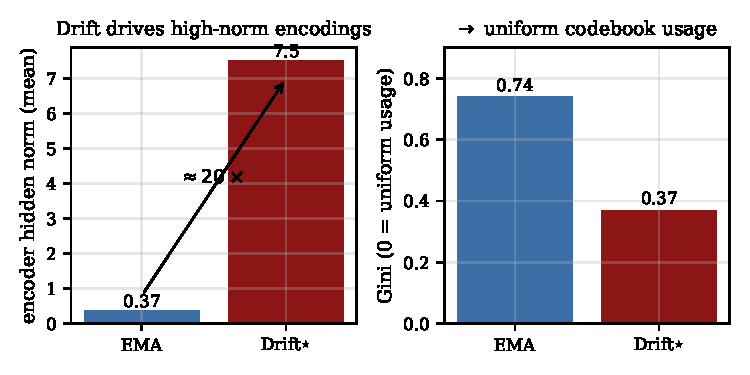
\includegraphics[width=0.95\linewidth]{figures/mechanism.pdf}
\caption{Mechanism on CIFAR-100, $K{=}512$. The energy produces encoders with large
pre-normalization feature norms (left), which sharpen the nearest-code assignment
and yield near-uniform codebook usage, reflected as a low Gini coefficient (right).}
\label{fig:mech}
\end{figure}

\subsection{The advantage grows with codebook size}

We next examine how performance changes as the codebook grows
(Figure~\ref{fig:scaling}, CIFAR-100). EMA's effective usage ppl/$K$ stays between $22$ and $37\%$ at every $K$, so a bigger
codebook buys only a few more usable codes, and at $K{=}8192$ utilization itself drops
to about $92\%$. Drift$\star$ holds ppl/$K$ near $80\%$ across the range we tested. PSNR
follows the same pattern. Drift$\star$ is ahead at every $K$, with the margin shrinking
from about $0.72$\,dB at $K{=}512$ to about $0.25$\,dB at $K{=}8192$.

\begin{figure*}[t]
\centering
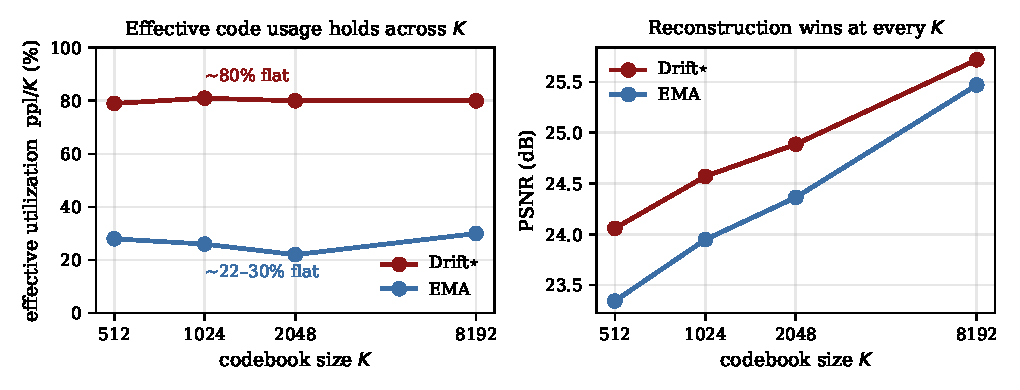
\includegraphics[width=0.75\linewidth]{figures/scaling.pdf}
\caption{Scaling across codebook size $K$ (CIFAR-100, $30$k iters; $K{=}8192$
uses stable seeds only). \textbf{Left:} effective utilization ppl/$K$. Drift$\star$
stays near $80\%$ while EMA stays near $22$--$30\%$, indicating the Zipfian
concentration is structural rather than a small-$K$ artifact. \textbf{Right:}
Drift$\star$ achieves higher reconstruction PSNR than EMA at every $K$ tested.}
\label{fig:scaling}
\end{figure*}

\subsection{The improvement generalizes across datasets}

Figure~\ref{fig:cross} collects the Drift$\star$ minus EMA gap across all four datasets
and several codebook sizes at $30$k iterations. The direction is the same everywhere,
with higher PSNR, lower FID, and $2.7$ to $4.0{\times}$ higher perplexity. If anything
the gains are a little larger on the harder, higher-class-count datasets, with the
biggest FID drop, $15.0$, on STL-10. This consistency is the main reason we think the
effect is a property of the quantizer rather than of one dataset, though all runs share
the same small encoder.

\begin{figure*}[t]
\centering
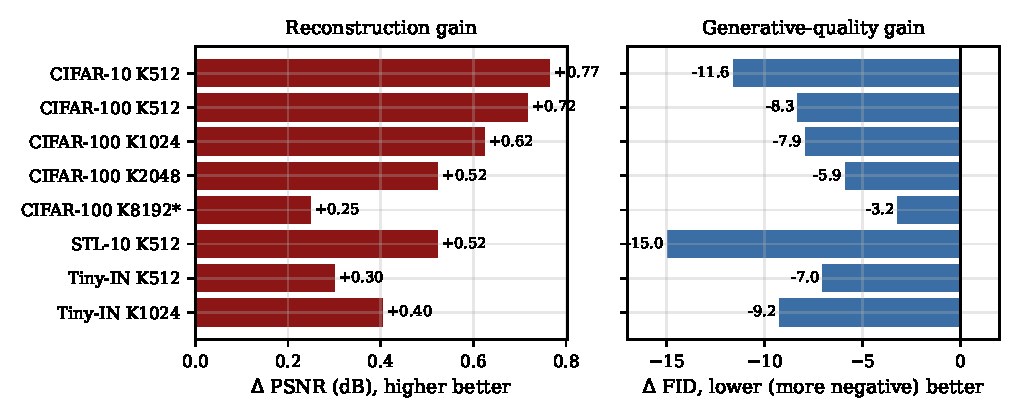
\includegraphics[width=0.80\linewidth]{figures/crossdata.pdf}
\caption{Generalization across datasets and codebook sizes ($30$k iters).
\textbf{Left:} PSNR improvement of Drift$\star$ over EMA (higher is better).
\textbf{Right:} FID reduction (more negative is better). The asterisk marks results
from stable seeds only; Tiny-IN $K{=}512$ EMA uses $n{=}2$.}
\label{fig:cross}
\end{figure*}

\section{Downstream Tasks}
\label{sec:downstream}

Reconstruction quality does not reveal whether the codes in the codebook are actually more useful. We test that in this section by applying DriftingVQ on two downstream tasks: recognition, where the frozen codes serve as features for classification, and generation, where they serve as the vocabulary for an autoregressive image prior. These are the two settings that tokenizer quality most directly affects. Qualitative inspection of the reconstructions in Figure~\ref{fig:recons} suggest that Drift$\star$'s advantage is in high-frequency detail, edges, sharp boundaries, and abrupt color changes. That is why we also run STL-10 at $64{\times}64$. At higher resolution there is more such detail to preserve, so differences between quantizers should be easier to see.

\subsection{Using the codes for recognition}
\label{sec:recognition}

Our first downstream question is whether the codes carry more class-relevant information. We freeze the trained encoder and codebook and train only a small head on top, so any difference comes from the frozen features. We run two probes of increasing capacity. The \emph{linear probe} uses a bag-of-codewords representation: the encoder maps each image to $8{\times}8{=}64$ code assignments, from which we form a normalized histogram over the $K$ codes, where entry $k$ counts how often code $k$ appears, analogous to a bag-of-words histogram in text. This $K$-dimensional vector is the input to a logistic regression on CIFAR-100. The \emph{CNN probe} instead trains a small convolutional head on the spatial latent grid, using both which codes appear and where.

Table~\ref{tab:recognition} reports both results. Drift$\star$ codes are modestly but
consistently more class-informative: the linear probe improves top-1 by $1.4$ points and
the CNN probe by roughly $0.63$, with every Drift$\star$ seed ahead of every EMA seed. For
reference, a CNN head on raw pixels reaches $54.1\%$ top-1 and a random frozen encoder
$13.4\%$, confirming that the codes carry real but compressed information. The gain is
consistent with the view that even usage lets each code specialize in a distinct visual
pattern, rather than forcing a few codes to represent many different patches. The effect
is small, and we do not over-interpret it.

\begin{table}[ht]
\centering\small
\begin{tabular}{lcc}
\toprule
CIFAR-100, $K{=}512$ & EMA & Drift$\star$\\
\midrule
Linear probe top-1 (\%)\,$\uparrow$ & 13.1 & \textbf{14.5}\\
Linear probe top-5 (\%)\,$\uparrow$ & 33.4 & \textbf{36.1}\\
CNN probe top-1 (\%)\,$\uparrow$ & 27.6\,$\pm$\,0.3 & \textbf{28.2\,$\pm$\,0.2}\\
CNN probe top-5 (\%)\,$\uparrow$ & 56.0\,$\pm$\,0.4 & \textbf{57.3\,$\pm$\,0.5}\\
\bottomrule
\end{tabular}
\vspace{2mm}
\caption{Recognition probes on frozen features (CIFAR-100, $K{=}512$; $3$ seeds for
CNN probe). Drift$\star$ codes are more class-informative under both probes. Reference:
$54.1\%$ top-1 for a raw-pixel CNN and $13.4\%$ for a random frozen encoder.}
\label{tab:recognition}
\end{table}

\subsection{Using the codes for generation}
\label{sec:generation}

Our second downstream question is whether the codes make a better vocabulary for an
image generator. We train a small autoregressive transformer prior over the code
sequences, sample new sequences, decode them through the frozen decoder, and measure
FID against the test set. We report two FID values to separate tokenizer quality
from prior quality. The \emph{reconstruction FID} decodes real test codes---the best
a perfect prior could achieve, isolating the tokenizer. The \emph{generation FID}
decodes codes sampled from the prior, measuring the full pipeline. Since FID is
sensitive to sampling temperature, we sweep and report the best value per method
(Figure~\ref{fig:fidtemp}).

Table~\ref{tab:generation} reveals an inherent trade-off. Drift$\star$'s codes are
harder to model: $6.72$ bits per code versus EMA's $5.59$, because a more uniform
distribution carries more entropy. One might therefore expect worse generation.
Instead, on CIFAR-100, the tokenizer quality advantage is large enough to dominate:
Drift$\star$ achieves lower reconstruction FID by $8.8$ and lower generation FID by
$11.6$. The prior also samples codes more evenly (sample Gini $0.47$ versus $0.78$),
which is closer to the training distribution. The generation advantage is smaller
than the reconstruction advantage, however, and depends on dataset and latent size
(Section~\ref{sec:stl10}); we therefore treat this as a result specific to our setup
rather than a general conclusion about generation quality.

\begin{table}[ht]
\centering\small
\begin{tabular}{lcc}
\toprule
CIFAR-100, $K{=}512$ & EMA & Drift$\star$\\
\midrule
Prior NLL (bits/code)\,$\downarrow$ & \textbf{5.59} & 6.72\\
Reconstruction FID\,$\downarrow$ & 65.8 & \textbf{56.9}\\
Generation FID\,$\downarrow$ & 91.1 & \textbf{79.6}\\
\bottomrule
\end{tabular}
\vspace{2mm}
\caption{Generation with an autoregressive prior (CIFAR-100, $K{=}512$, $3$ seeds).
Drift$\star$ codes are harder to model (higher NLL), yet the tokenizer quality
advantage is sufficient that both reconstruction FID and generation FID come out
lower. This reflects a reconstruction-versus-compressibility trade-off rather than
a free lunch.}
\label{tab:generation}
\end{table}

\begin{figure}[ht]
\centering
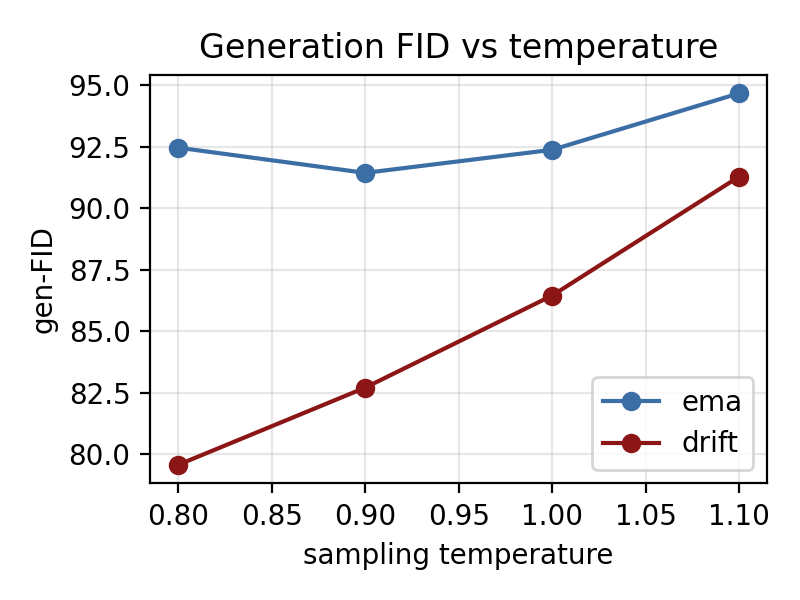
\includegraphics[width=0.85\linewidth]{figures/fid_vs_temp.png}
\caption{Generation FID as a function of sampling temperature (CIFAR-100,
$K{=}512$). FID is temperature-sensitive, so we sweep and report the best point per
method. Drift$\star$ achieves lower FID across the sampled range.}
\label{fig:fidtemp}
\end{figure}

\begin{figure*}[t]
\centering
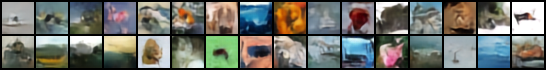
\includegraphics[width=\textwidth]{figures/samples_compare_cifar.png}
\caption{Samples decoded from trained priors (CIFAR-100, $K{=}512$), each at its best
sampling temperature. Top block: EMA prior. Bottom block: Drift$\star$ prior. The same
generator is used throughout, so the comparison isolates the tokenizer.}
\label{fig:samples}
\end{figure*}

\subsection{Higher-resolution results on STL-10}
\label{sec:stl10}

The CIFAR results above are at $32{\times}32$, where visual differences are subtle
(Figure~\ref{fig:recons}). We repeat the comparison on STL-10 at $64{\times}64$ with
a $16{\times}16$ latent grid, which preserves more spatial detail through the
bottleneck. Figure~\ref{fig:stl10} shows the result. At this resolution the fine-detail
advantage is more clearly visible, and the error map makes it explicit: EMA loses
more information along edges and textured regions, which appear brighter in the error
map, while Drift$\star$ remains darker in those areas. The recognition gap also
grows: the CNN probe reaches $54.9\,{\pm}\,0.9\%$ top-1 for Drift$\star$ versus
$51.8\,{\pm}\,0.5\%$ for EMA, a $3.0$-point gain with every Drift$\star$ seed beating
every EMA seed---roughly five times the CIFAR-100 gap.

The generation results on STL-10 sharpen the reconstruction-versus-compressibility
trade-off. The reconstruction FID gap is large: $55.1$ for Drift$\star$ versus $74.5$
for EMA, a $19.5$-point improvement. The generation FID gap is much smaller: $114.4$
versus $117.2$, only $2.9$ points. The $16{\times}16$ latent gives the prior $256$
tokens to model instead of $64$; the additional difficulty of modeling Drift$\star$'s
more uniform codes erodes most of the tokenizer advantage at this scale. Drift$\star$
still leads on both metrics, but this result makes clear that the generation benefit
is sensitive to latent sequence length and would require larger priors to fully
realize.

\begin{figure*}[t]
\centering
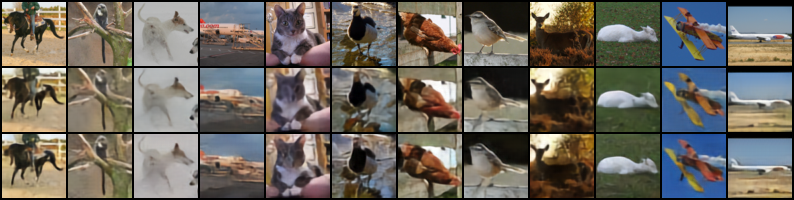
\includegraphics[width=\textwidth]{figures/recon_compare_stl10.png}\\[2mm]
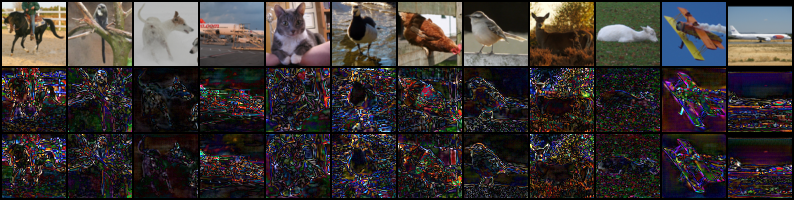
\includegraphics[width=\textwidth]{figures/recon_error_stl10.png}
\caption{Higher-resolution comparison on STL-10 ($64{\times}64$, $16{\times}16$ latent).
Top: reconstructions, with rows showing input, EMA, and Drift$\star$ on the same images.
Bottom: amplified absolute reconstruction error (brighter $=$ more error). EMA loses more
detail along edges and textures. Mean PSNR: $26.3$\,dB for EMA and $26.9$\,dB for
Drift$\star$.}
\label{fig:stl10}
\end{figure*}

\section{Limitations and Failure Modes}

We report two limitations beyond the intentionally small model scale of these
experiments.

\noindent\textbf{Stability at very large $K$.} At $K{=}8192$, one of three
Drift$\star$ seeds collapsed, reaching PSNR $22.8$ with only $61\%$ of codes active,
while EMA was stable on all three. The remaining two Drift$\star$ seeds were stable
and outperformed EMA. A reduced energy weight did not reliably prevent the collapse,
so large-$K$ stability remains an open problem.

\noindent\textbf{Prior compressibility.} As shown in Section~\ref{sec:generation},
Drift$\star$ codes cost approximately $1.1$ extra bits per code under an
autoregressive prior. This did not erase the generation gain on CIFAR-100, but it
is a genuine trade-off that becomes more consequential as the latent sequence grows
longer (Section~\ref{sec:stl10}) and could matter more at larger scale.

The autoencoder is intentionally small---an $8{\times}8{\times}64$ latent and $30$k
training iterations---to support the large ablation, seed, and dataset matrix.
Absolute PSNR and FID values fall well below those of adversarially-trained,
full-scale tokenizers and should be read as controlled comparisons rather than
state-of-the-art benchmarks.

\section{Conclusion}

Our project studied whether a physics-inspired VQ-VAE, validated only on
two-dimensional synthetic data, transfers to deep convolutional networks and real
images. The original formulation trails the EMA baseline, but after removing the hidden-to-hidden repulsion term
and replacing the rotation-trick gradient with a straight-through estimator, we found a
resulting Drift$\star$ which improves reconstruction, perceptual quality, and codebook usage
altogether. Across four datasets, we found the gap widening as the codebook grows, which is
where standard quantizers waste the most capacity. We trace this to an emergent large
encoder norm that sharpens code assignments. Downstream, the codes give a consistent
recognition gain and also help generation, though the generation benefit is sensitive
to latent size and needs larger priors to realize fully.

These results indicate that uniform codebook usage and strong reconstruction need not
conflict, at least at the scales we studied. Two extensions follow. First, applying
Drift$\star$ within a full-scale tokenizer with perceptual and adversarial losses would
test whether the reconstruction advantage carries to tasks such as detection,
segmentation, and retrieval. Second, large-$K$ stability and the
reconstruction-versus-compressibility trade-off remain open; an adaptive energy schedule
or a light entropy penalty on the prior may help recover the best of both.

{\small
\bibliographystyle{ieee}
\bibliography{egbib}
}

\section*{Contributions and Acknowledgements}

\noindent\textbf{Hemal Arora} led problem formulation, DriftingVQ implementation, the ablation study, and the main experimental program through cross-dataset generalization.
\textbf{Tesvara Jiang} led downstream generation experiments, report writing, and literature review.
\textbf{Ethan Zhang} contributed to problem formulation, literature review, downstream CNN probe experiments, and exploratory work with non-natural image datasets.

\medskip
\noindent\textbf{Generative AI Usage.}
Claude Code CLI (\texttt{claude-sonnet-4-6}, Anthropic) was used extensively for code generation: the experiment harness, training loop, model definitions, evaluation scripts, and Modal GPU orchestration were largely written by Claude. The \texttt{DriftingVQ} module was implemented by Claude from the team's physics-energy specification. Claude also helped with ideation and debugging throughout. Report prose was written by the team. A detailed breakdown is in \texttt{AI\_USAGE.md} at the repository root.

\end{document}
